
%%%%%%%%%%%%%%%%%%%%%%%%%%%%%%%%%%%%%%%%%%%%%%%%%%%%%%%%
%GRASS PROMOTION FLYER                                 %
%(c) 2007 GRASS PROMOTION TEAM                         %
%GNU Free Documentation License                        %
%Version 1.2                                           %
%Needs leaflet.cls				       %
%www.ctan.org/tex-archive/macros/latex/contrib/leaflet/%
%%%%%%%%%%%%%%%%%%%%%%%%%%%%%%%%%%%%%%%%%%%%%%%%%%%%%%%%

%Sometimes printing engines need the 2nd side upside down
%in this case, use tumble (which is default) instead of notumble
%If this causes problems, use notumble
%If you need a foldmark, delete nofoldmark
\documentclass[notumble,a4paper,10pt,nofoldmark]{leaflet}
\usepackage[latin1]{inputenc}
\usepackage[T1]{fontenc}
\usepackage[ngerman]{babel}
\usepackage{helvet,courier,xcolor}

% Set Helvetica as the default font
\renewcommand*\familydefault\sfdefault
% Let LaTeX knows that pictures are found in ./pix
\graphicspath{{pix/}}

% Setting up things for the captions
\usepackage{caption}[2004/07/16]
\captionsetup{%
  font={small,it},%
  labelformat=empty,% Leaves out label: ``Figure 1''
  labelsep=none,%
  aboveskip=0pt%
}
% Defining a new 'figure' environment for the document
\newenvironment{myfig}[1][0pt plus 1.5ex minus .5ex]{\par\vspace*{#1}\begin{minipage}{\textwidth}\centering}{\end{minipage}}

% Defining the GRASS homepage
\newcommand{\GRASSurl}{\url{http://grass.osgeo.org}}

% Define a color for the URIs
\definecolor{darkblue}{RGB}{0,0,88}

\usepackage{hyperref}
% Setting up some document info
\hypersetup{%
  colorlinks=true,%
  urlcolor=darkblue,% Redefine this color to change URIs color
  pdfauthor={The GRASS Community},%
  pdftitle={GRASS GIS: Efficiency through Freedom \& Transparency},%
  pdfsubject={GRASS Promotion Flyer},%
  breaklinks=true,%
  plainpages=false%
}

% Title page stuff
\title{\textbf{\huge GRASS GIS}\\%
\textsl{Efficiency through Freedom \& Transparency}}
\author{Die GRASS Community}
\date{
\includegraphics[width=\textwidth]{grasslogo_vector}\\[2ex]
\large\GRASSurl}

\begin{document}

\maketitle
\thispagestyle{empty}% Necessary to leave out the page number on the first page

\newpage

\section{Was ist GRASS}

GRASS (Geographic Resources Analysis Support System) ist eine frei verf"ugbare Software f"ur ra"umliche Analysen, deren Quellcode f"ur jeden uneingeschr"ankt zug"anglich ist. Es besteht aus mehr als 350 Modulen um Vektor (2D/3D), Raster und Voxeldaten zu prozessieren. Eine Vielzahl von Schnittstellen zu anderen Softwarepacketen in affinen Bereichen wie Geostatistik, Datenbanken, Kartenservern und sogar zu anderen GIS- Programmen existieren. Es ist das gr"o�te Open Source GIS. Man kann es als Desktop- GIS einsetzen und es kann als R�ckgrad einer kompleten GIS- Infrastruktur dienen.   

\section{Wo wird GRASS eingesetzt}
GRASS wird erfolgreich in Forschung, Wirtschaft und in "offentlichen Verwaltungen eingesetzt. GRASS hat weltweit in einer Vielzahl von Anwendungen sein gro"ses Potential zur Durchf"uhrung r"aumlicher Analysen gezeigt.

\section{Zur Geschichte von GRASS}
GRASS wurde Anfang der 90'er vom US ARMY Construction Engineering Research Laboratories (USA-CERL) entwickelt und lizenzfrei ver"offentlicht. Als sich das USA-CERL aus der Entwicklung zur"uckzog, wurde diese Aufgabe von einem internationalen Entwicklerteam "ubernommen. Seit 1999 wird GRASS als Freie Software unter den Bedingungen der GNU General Public Licence (GPL) ver"offentlicht.
\begin{myfig}
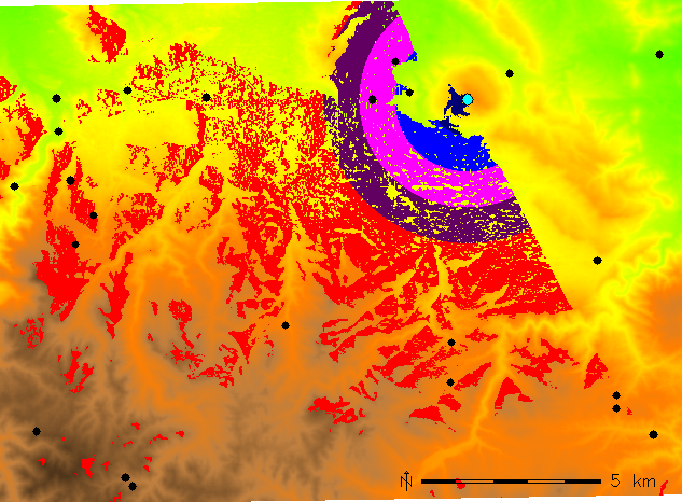
\includegraphics[width=0.6\textwidth]{visibility}
\captionof{figure}{Sichtbarkeitsanalyse in GRASS}
\end{myfig}

\section{Open Source Philosophie}
Die Open Source Philosophie gibt dem Anwender die M"oglichkeit, den Quellcode und die Struktur eines Programmes einzusehen. Dies bietet ein hohes Ma"s an Transparenz. Jeder kann das Programm auf seine Bed"urfnisse hin erweitern. Um eine hohe Qualit"at zu gew"ahrleisten, findet eine unmittelbare Durchsicht des Quellcodes statt. Mit Hilfe des Extension Managers k"onnen eigene Module ohne GRASS- Quellcode erstellt werden.

\section{Technische Daten}

\subsection{Lizenz}

GNU General Public License (Free Software Foundation)

\subsection{Unterst"utzte Plattformen}

GRASS l"auft auf fast allen Plattformen. GNU/Linux, Posix konformen Unix Systemen, MS-Windows \& Mac\-OS X.

\subsection{Design}

\begin{itemize}
\item Modular, GRASS besteht aus mehr als 350 Modulen
\end{itemize}

\subsection{Programmiersprachen}

\begin{itemize}
\item ANSI C
\item GRASS- SWIG Interface
\item Python f"ur WebGIS Applikationen
\item Java Version: JGRASS
\end{itemize}

\subsection{Datenmanagement }

\begin{itemize}
\item Raster-,  Vektor-, Voxeldaten
\item 2D / 3D Raster-, Vektormodellierung
\item Bildverarbeitung
\item Vektortopologien / Netzwerkanalysen
\item Geostatistik (Schnittstelle zu R)
\end{itemize}

\begin{myfig}[1ex]
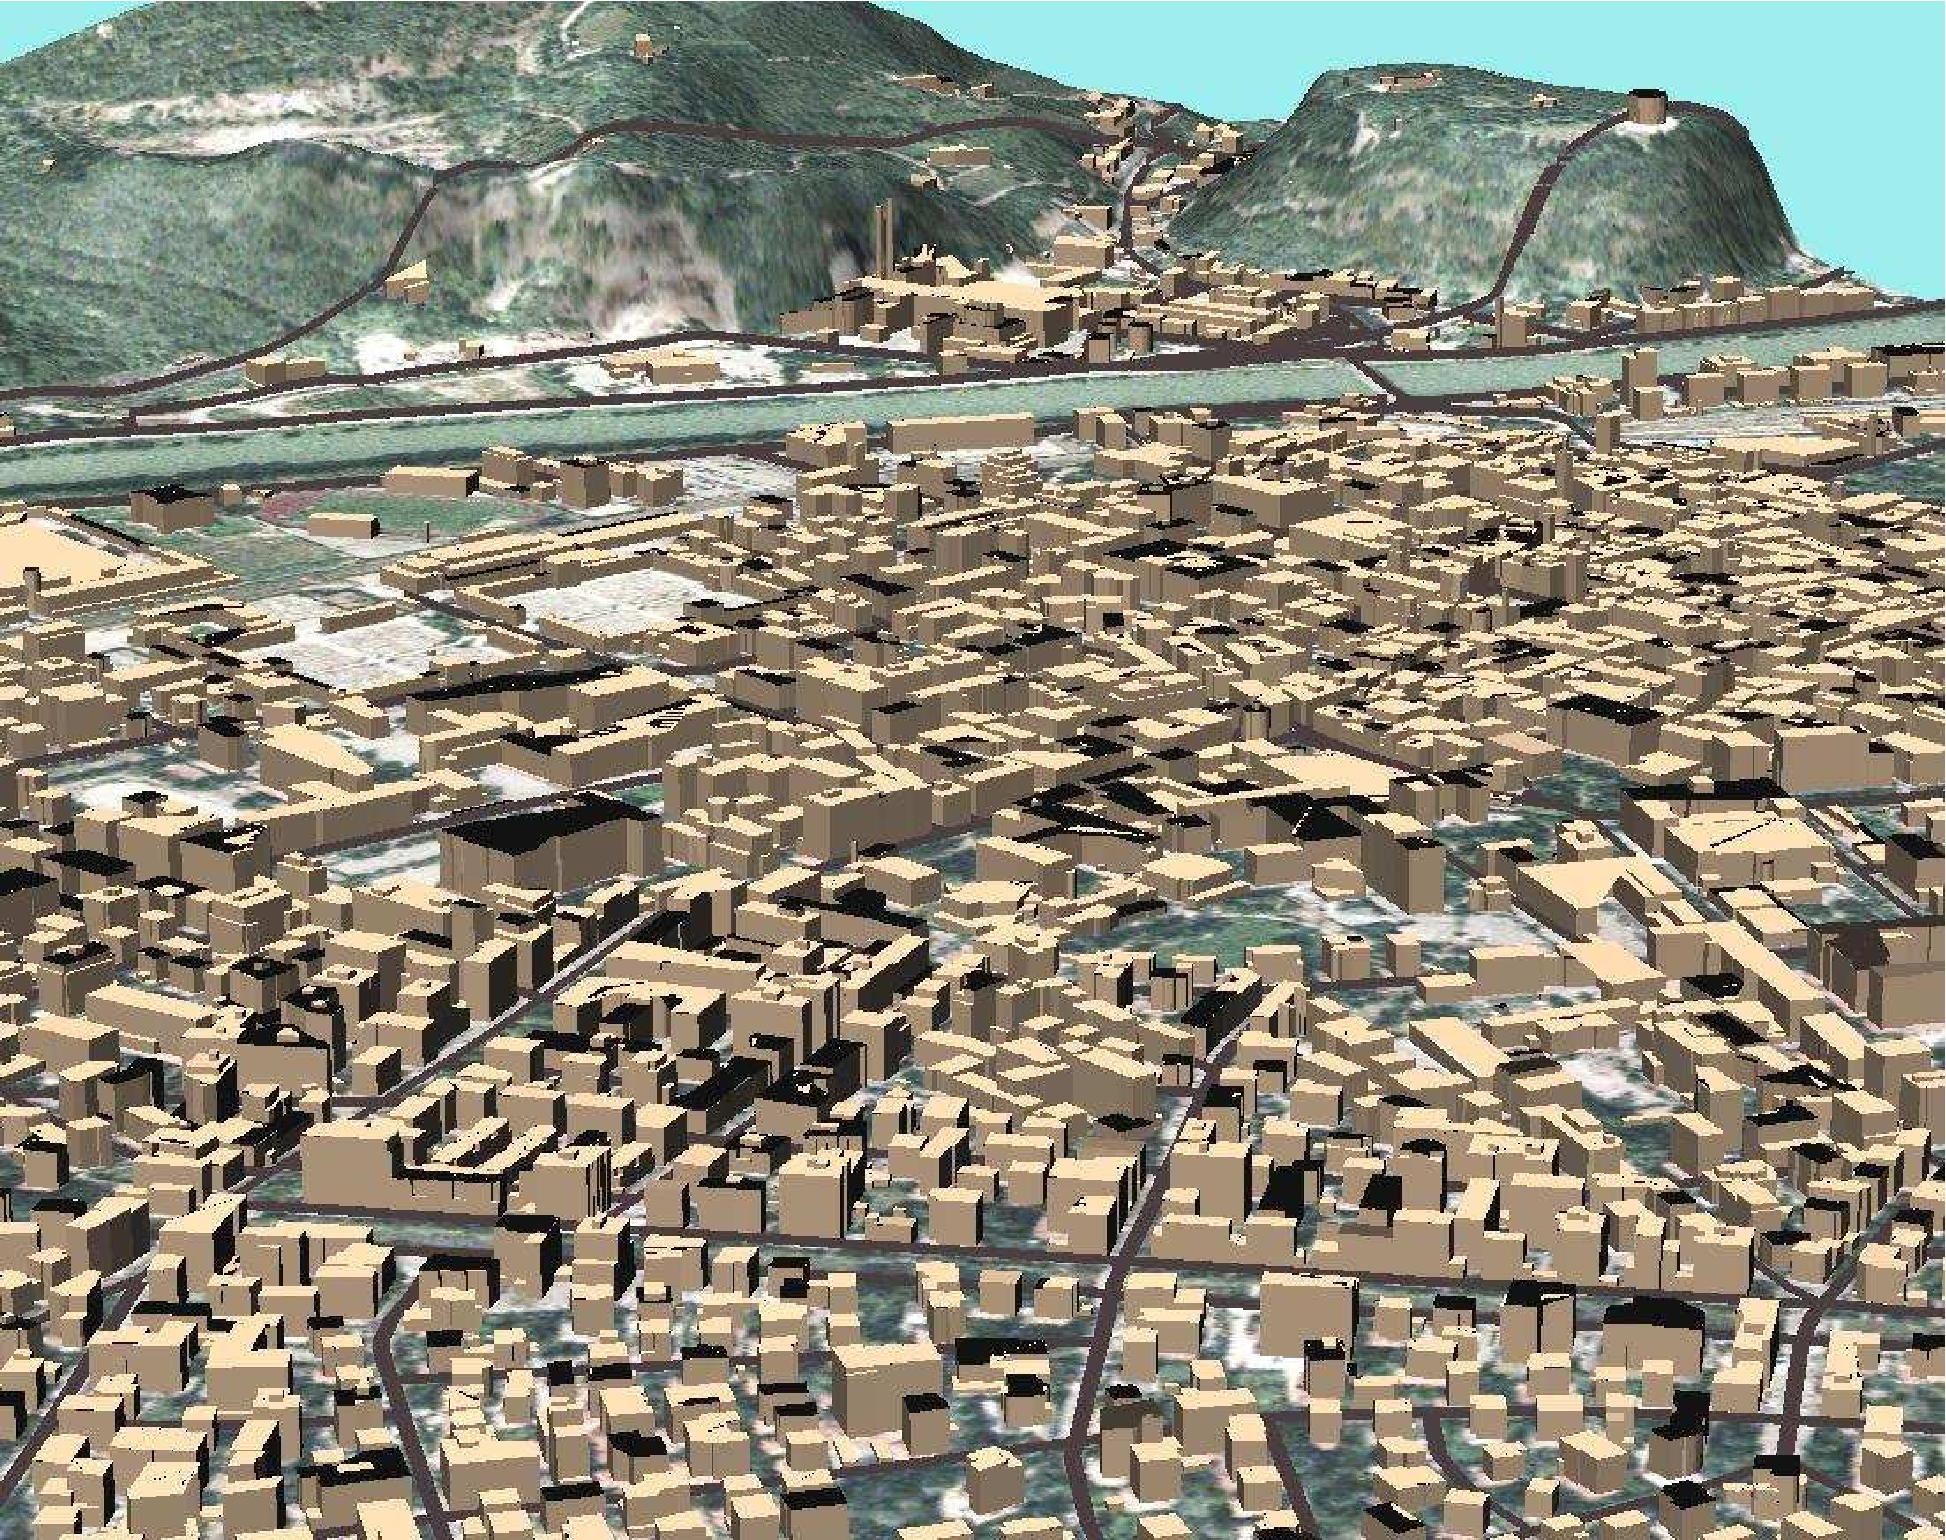
\includegraphics[width=0.6\textwidth]{trento3d}
\captionof{figure}{3D Ansicht von Trient, Italien}
\end{myfig}

\section{Unterst"utzte Dateiformate}
GRASS unterst"utzt fast alle g"angigen GIS- Formate, da es die GDAL/OGR Bibliothek benutzt. Au"serdem unterst"utzt es OGC Simple Features.

\subsection{Unterst"utzte Vektorformate}
ASCII, ARC/INFO ungenerate, ARC/INFO E00, Arc\-View SHAPE, BIL, DLG (U.S.), DXF, DXF3D, GMT, GPS-ASCII USGS-DEM, IDRISI, MOSS, MapInfo MIF, PostGIS, TIGER, VRML, \dots

\subsection{Unterst"utzte Rasterformate}
ASCII, ARC/GRID, E00, GIF, GMT, TIF, PNG, Vis5D, SURFER (.grd),\dots
\begin{myfig}
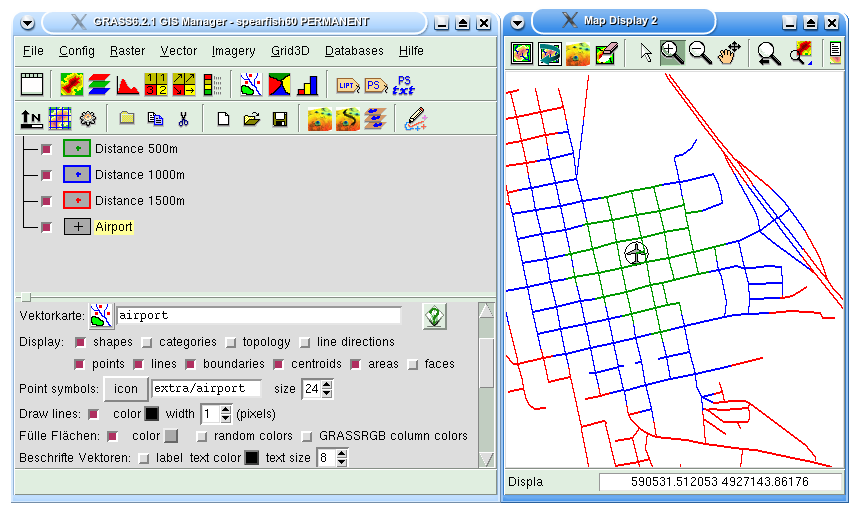
\includegraphics[width=0.6\textwidth]{isodist}
\captionof{figure}{Netzwerkanalyse und GRASS GUI}
\end{myfig}

\subsection{Unterst"utzte Bildformate}

CEOS (SAR, SRTM, LANDSAT7 etc.), ERDAS LAN / IMG, HDF, LANDSAT TM/MSS, NHAP aerial photos, SAR, SPOT, \dots
\begin{myfig}[1.5ex]
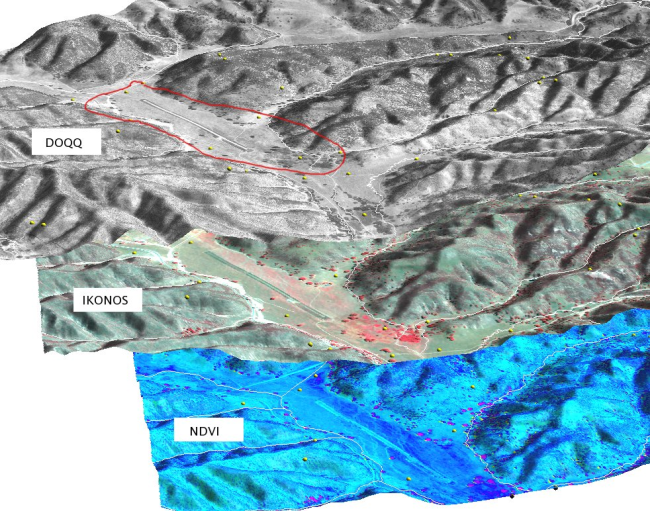
\includegraphics[width=0.6\textwidth]{ndvi}
\captionof{figure}{Bildverarbeitung in GRASS}
\end{myfig}

\subsection{Datenbanken}

\begin{itemize}
\item PostgreSQL / PostGIS
\item MySQL
\item SQLite
\item ODBC 
\item DBF
\end{itemize}

\subsection{Ausgabe}

\begin{itemize}
\item Module, um Karten zu erstellen
\item NVIZ um 2.5D und 3D Daten zu visualisieren (Animationen \& Flybys)
%\item{GMT export}
%item{VRML}
\item VTK, POVray
\item WebGIS via Mapserver, Python, etc.
\end{itemize}

\subsection{Interoperabilit"at mit anderer Software}

\begin{itemize}
\item Quantum GIS (Freier Geodaten Viewer und mehr)
\item R- Language (Statistik)
\item Gstat (Geostatistik)
\item UMN Mapserver (Webmapping)
\end{itemize}

\section{Wo finden Sie mehr Informationen}

\begin{itemize}
%\begin{flushleft}
\item{Website: \\\GRASSurl}
\item{GRASS Wiki: \\\url{http://grass.osgeo.org/wiki}}
%\item{GRASS Promotion Team: \\\url{malte@perlomat.de}}
\item{GRASS Mailingliste: \\\url{http://grass.osgeo.org/community/support.php}}
\item{Deutsche Grass Mailingliste: \\\url{https://grass-verein.de/mailman/listinfo/gav-talk}}
%\end{flushleft}
\end{itemize}

\section{GRASS Anwender Vereinigung e. V.}
In Deutschland bietet die GRASS Anwendervereinigung e.V., die sich die F"orderung und Verbreitung freier GIS Software zum Ziel gesetzt hat, ein Forum f"ur Fragen rund um GRASS und freier GIS Software allgemein.
\begin{center}

\includegraphics[width=0.5\textwidth]{Logo_GAV}\\
\url{http://www.grass-verein.de}
\end{center}
\section{OSGeo}
GRASS ist ein Gr"undungsprojekt der Open Source Geospatial Foundation, die sich das Ziel gesetzt hat, qualitativ hochwertige Open Source Geo- Software zu entwickeln. F"ur weitere Informationen besuchen Sie bitte die OSGeo Homepage:
\begin{center}

\includegraphics[width=0.5\textwidth]{OSGeo_CMYK}\\
\url{http://www.osgeo.org}
\end{center}

\end{document}
